% This example is meant to be compiled with lualatex or xelatex

% The theme itself also supports pdflatex
\PassOptionsToPackage{unicode}{hyperref}
\documentclass[aspectratio=1610, 9pt]{beamer}

% Load packages you need here
\usepackage{polyglossia}
\setmainlanguage{german}
\usepackage[font=small,labelfont=bf]{caption}
\usepackage{csquotes}
\usepackage{siunitx}
\usepackage{subfigure}

\usepackage{amsmath}
\usepackage{amssymb}
\usepackage{mathtools}

\usepackage{hyperref}
\usepackage{bookmark}

% load the theme after all packages

\usetheme[
  showtotalframes, % show total number of frames in the footline
]{tudo}

% Put settings here, like
\unimathsetup{
  math-style=ISO,
  bold-style=ISO,
  nabla=upright,
  partial=upright,
  mathrm=sym,
}

\title{Entwicklung eines Programmes zur Berechnung von Annealingeffekten in bestrahltem Silizium nach dem Hamburger Modell}
\author[C.~Krause]{Christopher Krause}
\institute[E4]{Experimentelle Physik \\ Fakultät Physik}
\titlegraphic{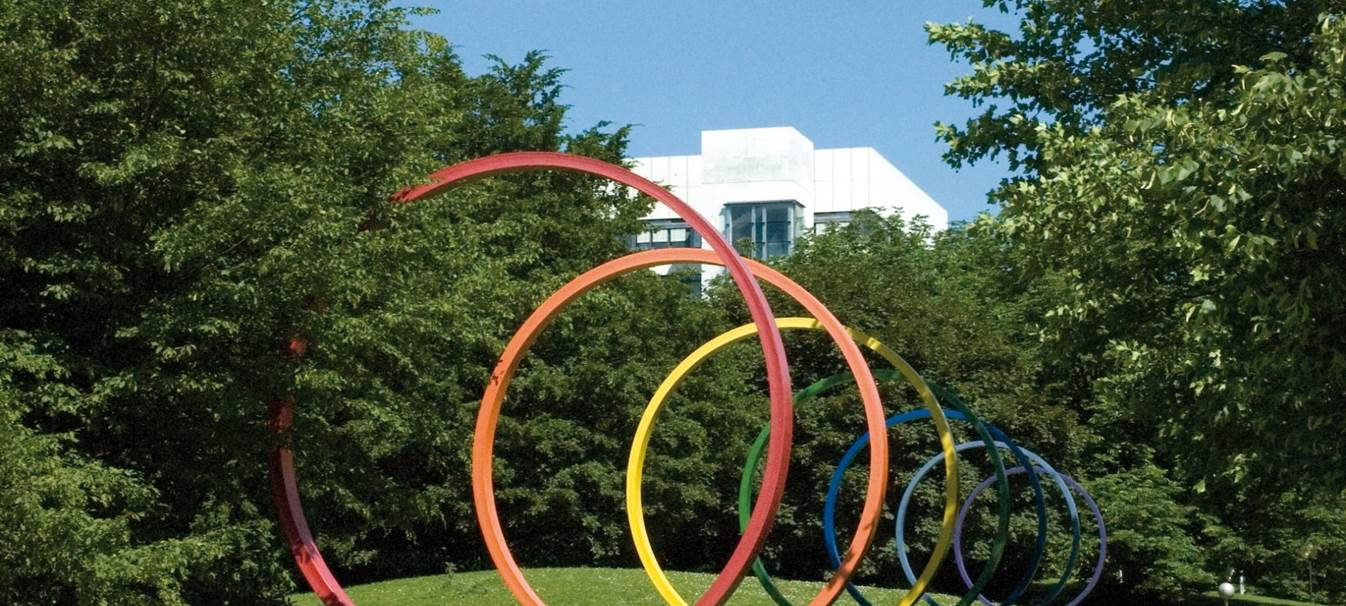
\includegraphics[width=0.7\textwidth]{images/tudo-title-2.jpg}}


\begin{document}

\maketitle




\begin{frame}{Motivation}
  \begin{itemize}
    \item Siliziumdetektoren finden unter anderem in Hochenergiephysik Verwendung
    \medskip
    \item Werden für Bestimmung von Ladung und Impuls in Experimenten wie ATLAS benötigt
      \begin{itemize}
        \item Pixeldetektoren im Inner Tracker
        \item Streifendetektoren im Semiconductor Tracker
      \end{itemize}
    \medskip
    \item Hervorgerufene Strahlenschäden durch Detektion von Teilchen führt zur Beschädigung des Detektors
      \begin{itemize}
        \item Erhöhung des Leckstromes
        \item Änderung der effektiven Dotierungskonzentration
      \end{itemize}
    \medskip
    \item Für lange Lebenszeit der Detektoren ist Untersuchung der Strahlenschäden und
          deren Behebung wichtig
  \end{itemize}
\end{frame}



\begin{frame}{Strahlenschäden}
  \begin{itemize}
    \item Entstehen durch Wechselwirkung von einfallenden Teilchen mit Detektormaterial
    \medskip
    \item Über Ionisation abgegebene Energie führt zu keinen Schäden im Detektor
    \medskip
    \item Streuung der Strahlung an Atomkernen im Bulk führt zu Defekten
      \begin{itemize}
        \item Atomkern wird aus Gitter herausgeschlagen $\rightarrow$ Zwischengitteratom
        \item Fehlendes Atom im Gitter $\rightarrow$ Leerstelle
      \end{itemize}
    \medskip
    \item Defekte führen zu Änderung der effektiven Dotierungskonzentration
    \medskip
    \item Generation von Ladungsträger an Defekten führt zu größerem Leckstrom
  \end{itemize}
\end{frame}




\begin{frame}{Annealing}
  \begin{itemize}
    \item Beschreibt durch Erhitzung hervorgerufene Änderungen von Materialeigenschaften
    \medskip
    \item Durch annealing von Defekten können verschiedene Effekte aufteten
      \begin{itemize}
        \item Migration: Für hohe Temperaturen wandern Zwischengitteratome durch Gitter und
        können Leerstellen füllen
        \medskip
        \item Komplexformation: Mehrere Zwischengitteratome können sich durch Migration Gruppieren und Komplexe formen
        \medskip
        \item Komplexe und Fehlstellen können bei hohen Temperaturen dissozieren, wodurch einzelne Bestandteile durch das Gitter wandern
      \end{itemize}
    \medskip
    \item Manche Komplexe sind stabil und werden durch annealing nicht beeinflusst
  \end{itemize}
\end{frame}


\begin{frame}{Ziel der Bachelorarbeit}
  Für beliebige Zeiten, Temperaturverläufe, Fluenzen und Materialeigenschaften:
  \begin{itemize}
    \item Berechnung der Dotierungskonzentration $\Delta N_{\mathrm{eff}}$
    \item Berechnung der Schadensrate $\alpha$
  \end{itemize}
  \medskip

  Zusätzliche Aufgaben:
  \begin{itemize}
    \item Interpolation der Daten für mehr und genauere Werte
    \item Erstellung eines Interfaces zur schnellen Berechnung von $\Delta N_{\mathrm{eff}}$ und $\alpha$
    für konstante Temperaturen
    \item Zusammenfügen von Datendateien und Anpassung der zugehörigen Zeiten
    \item Gesamte Annealinghistorie einer Diode berechnen
  \end{itemize}
\end{frame}




\begin{frame}{Theoretische Grundlage: Das Hamburg Modell}
  Die Änderung der Dotierungskonzentration beim annealing wird durch 3 Terme beschrieben:
  \medskip
  \begin{itemize}
    \item Stable damage:\: $N_{\mathrm{C}}(\Phi_{\mathrm{eq}}) = \underbrace{ N_{\mathrm{C0}}[1-\exp{(-c \cdot \Phi_{\mathrm{eq}})}] }_{\text{Entfernung von Donatoren}} + \underbrace{ g_{\mathrm{c}} \cdot \Phi_{\mathrm{eq}} }_{\text{stabile Defekte}}$
    \medskip
    \item Shortterm annealing:\: $N_{\mathrm{A}}(t, \Phi_{\mathrm{eq}}, T)= \underbrace{ \Phi_{\mathrm{eq}} \cdot g_{\mathrm{a}} \cdot \exp{(-\frac{t}{\tau_{\mathrm{a}}})} }_{\text{Annealing von Akzeptoren}}$
    \medskip
    \item Longterm annealing:\: $N_{\mathrm{Y}}(t, \Phi_{\mathrm{eq}}, T)= \underbrace{\Phi_{\mathrm{eq}} \cdot g_{\mathrm{Y}} \cdot \left(1-\frac{1}{1+\frac{t}{\tau_{\mathrm{Y}}}}\right)}_{\text{Einführung von Akzeptoren}}$
    \medskip

    \item   $\Delta N_{\mathrm{eff}} = N_{\mathrm{C}}(\Phi_{\mathrm{eq}}) + N_{\mathrm{A}}(t, \Phi_{\mathrm{eq}}, T) + N_{\mathrm{Y}}(t, \Phi_{\mathrm{eq}}, T)$
  \end{itemize}
  \hfill
  \begin{minipage}[b]{0.35\linewidth}
    \vspace{-3cm} \hspace{-1.5cm}
  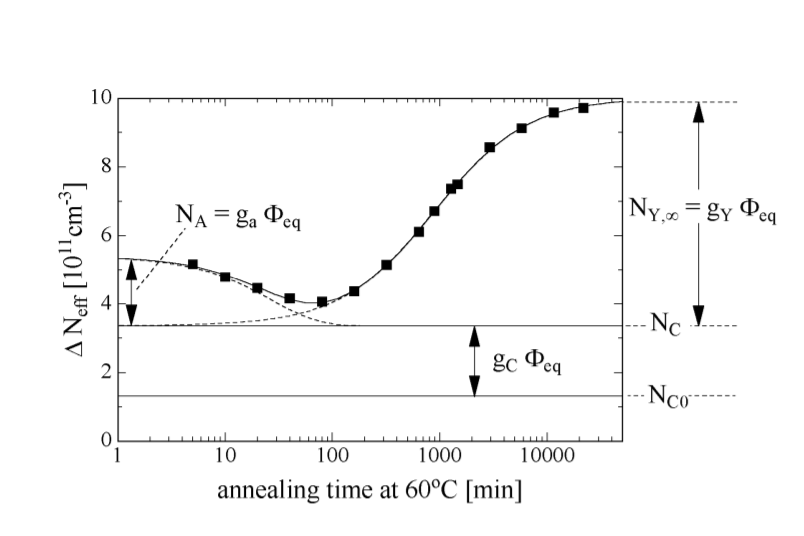
\includegraphics[height=12\baselineskip]{images/n_eff_beispiel.png}
  \captionof{figure}{$\Delta N_{\mathrm{eff}}$ für eine Fluenz von $1,4\cdot 10^{13} \, \mathrm{n_{eq}/cm^2}$.}
  \end{minipage}
\end{frame}

\begin{frame}{Theoretische Grundlage: Das Hamburg Modell}
  Durch Strahlung hervorgerufener Leckstrom: \:$\Delta I = \alpha \Phi_{\mathrm{eq}} \cdot V $ \\
  \medskip
  Die Schadensrate wird bei annealing durch 2 Terme beschrieben:
  \medskip
  \begin{itemize}
    \item Shortterm annealing:\: $\underbrace{\alpha_I \cdot \exp{\left(-\frac{t}{\tau_{\mathrm{I}}(T)}\right)}}_{\text{Annealing von Akzeptoren}}$
    \medskip
    \item Longterm annealing:\: $\underbrace{\alpha_{\mathrm{0}}^{*} -\beta \cdot \ln{\left(\Theta(T) \cdot \frac{t}{t_{\mathrm{0}}}\right)}}_{\text{Physikalisches Modell unklar}}$, \:\:\: mit \: $\Theta(T) = \frac{E_{\mathrm{I}}^*}{k_b} \exp{\left(-\frac{1}{T}-\frac{1}{T_{\mathrm{ref}}}\right)}$
    \medskip
    \item $\alpha(t, T) = \alpha_I \cdot \exp{\left(-\frac{t}{\tau_{\mathrm{I}}(T)}\right)} + \alpha_{\mathrm{0}}^{*} -\beta \cdot \ln{\left(\Theta(T) \cdot \frac{t}{t_{\mathrm{0}}}\right)}$
  \end{itemize}
  \medskip
  \hfill
  \begin{minipage}[b]{0.35\linewidth}
    \vspace{-1cm} \hspace{-2cm}
  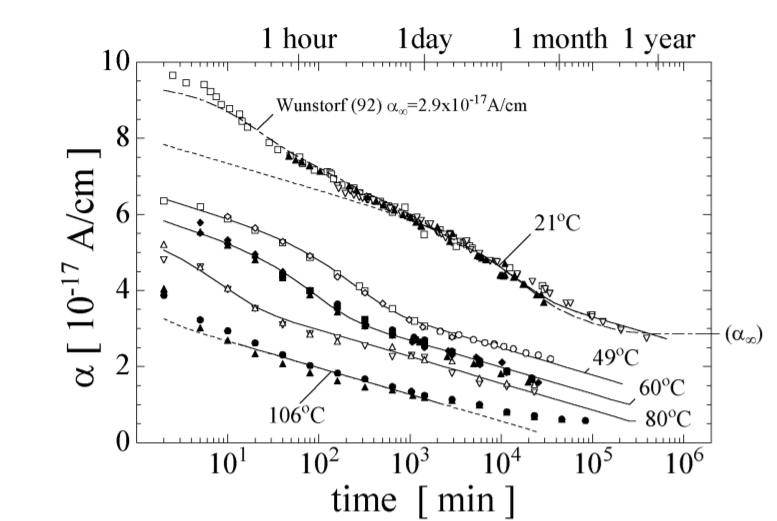
\includegraphics[height=11\baselineskip]{images/schadensraten.png}
  \end{minipage}
\end{frame}

\begin{frame}{Dotierungskonzentration für konstante Temperatur}
  \begin{figure}
      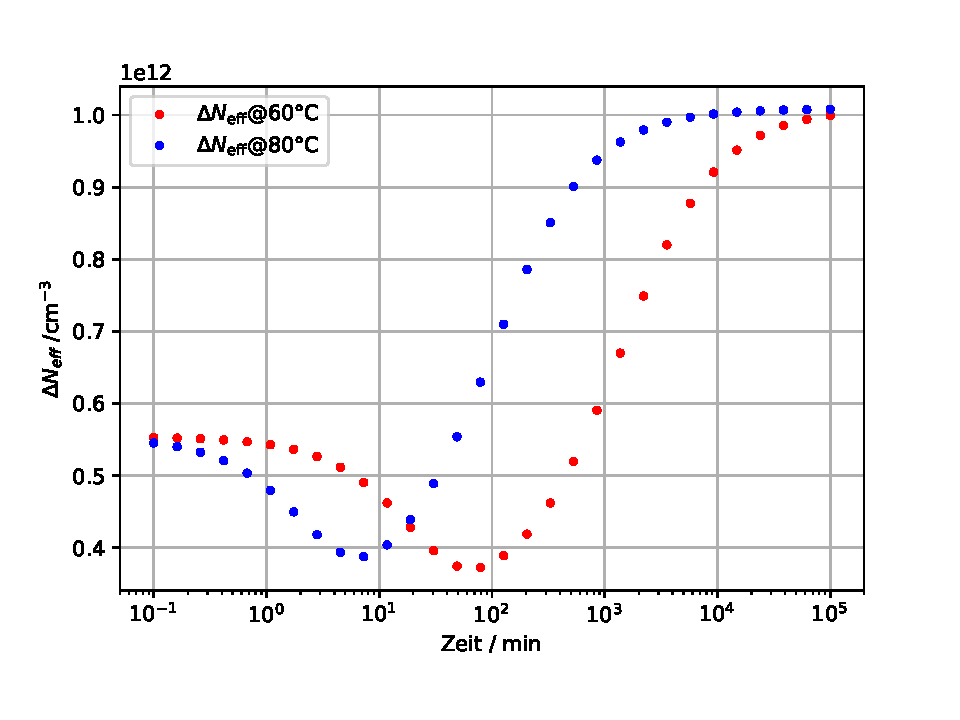
\includegraphics[width=0.55\textwidth]{images/annealing.PDF}
  \caption{$\Delta N_{\mathrm{eff}}$ einer WE-25k Diode nach einer Bestrahlung mit einer Fluenz von
    $5\cdot 10^{15} \, \mathrm{n_{\mathrm{eq}}/cm^2}$.}
  \end{figure}
\end{frame}

\begin{frame}{Schadensrate für konstante Temperatur}
  \begin{figure}
      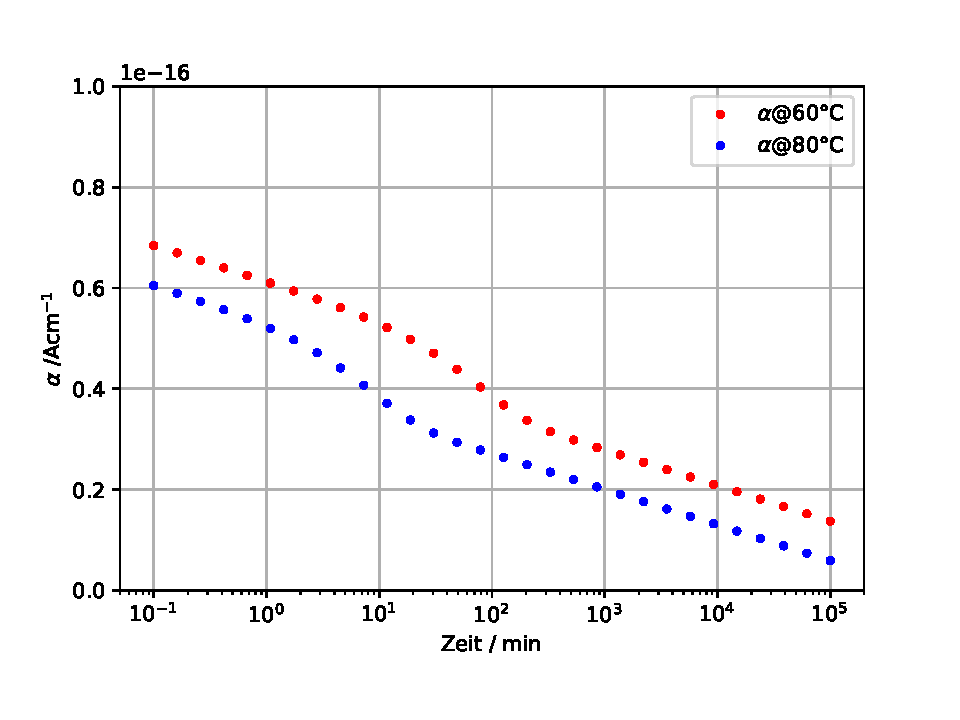
\includegraphics[width=0.55\textwidth]{images/damage.PDF}
  \caption{Schadensrate einer WE-25k Diode.}
  \end{figure}
\end{frame}


\begin{frame}{Analoge Berechnung für eine Temperaturkurve}
  \begin{itemize}
    \item Aufgenommene Temperaturkurve des Sensors R1 in Sandia
  \end{itemize}
  \begin{figure}
      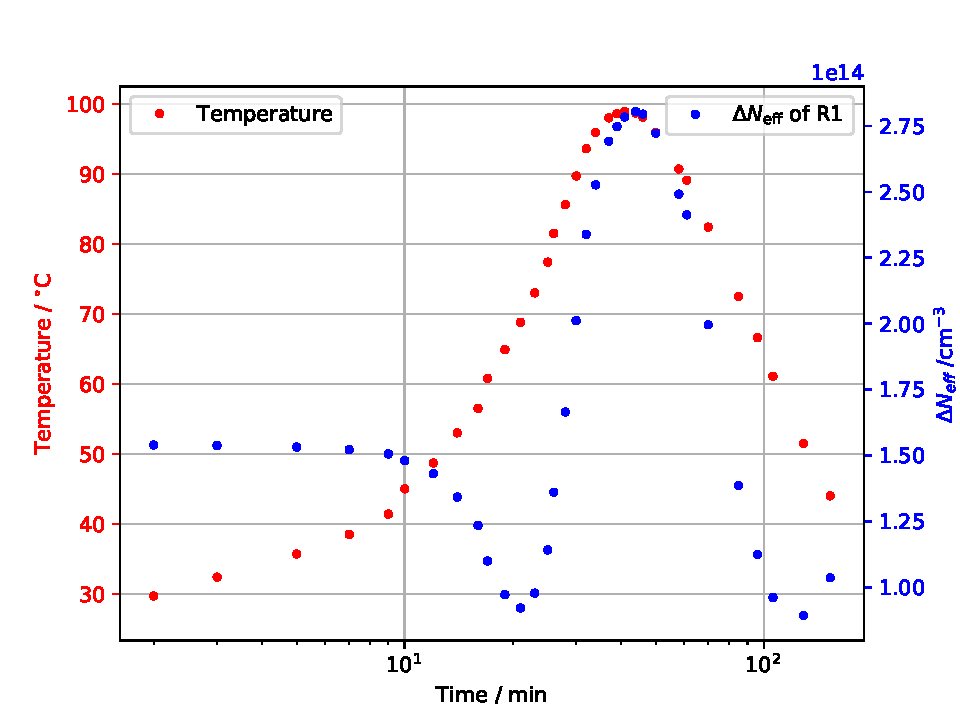
\includegraphics[width=0.5\textwidth]{images/ohnekorrektur.PDF}
  \caption{Dotierungskonzentration bei gleicher Fluenz und nicht konstanter Temperatur.}
  \end{figure}
\end{frame}

\begin{frame}{Korrekturansatz}
  \begin{itemize}
    \item longterm annealing weist klare Abweichung vom eigentlichen Verhalten auf
    \medskip
    \item vorherige Temperaturänderungen werden vernachlässigt
    \medskip
    \item Funktion kann nur mit konstanter Temperatur rechnen
  \end{itemize}
  \medskip
  $\rightarrow$ Korrektur wird benötigt
  \medskip

  Ansatz: Über den Zeitraum $t_{\mathrm{i}} - t_{\mathrm{i-1}}$ wird mit der Temperatur $\frac{T_{\mathrm{i}} +T_{\mathrm{i-1}}}{2}$ erhitzt.

  Für den shortterm annealingeffekt gilt beispielsweise:
  \begin{align*}
    &\frac{t_{\mathrm{n}}}{\tau_{\mathrm{a}}(T_{\mathrm{n}})} \rightarrow \sum_{i=0}^n  \frac{t_{\mathrm{i}} - t_{\mathrm{i-1}}}{\tau_{\mathrm{a}}(\frac{T_{\mathrm{i}} +T_{\mathrm{i-1}}}{2})} \:\:\:\: \text{für} \: n>0 \\
    \\
    &\text{mit} \:\:\:\:\:\: \tau_{\mathrm{a}}(T) \propto \frac{1}{\exp{\left(-\frac{1}{T}\right)}} \\
    \\
    &\text{und}  \:\:\:\:\:\: N_{\mathrm{A}}(t, \Phi_{\mathrm{eq}}, T)     \propto \Phi_{\mathrm{eq}} \cdot \exp{\left(-\frac{t}{\tau_{\mathrm{a}}(T)}\right) }
  \end{align*}
\end{frame}

\begin{frame}{Dotierungskonzentration mit Korrektur}
  \begin{figure}
      \subfigure[]{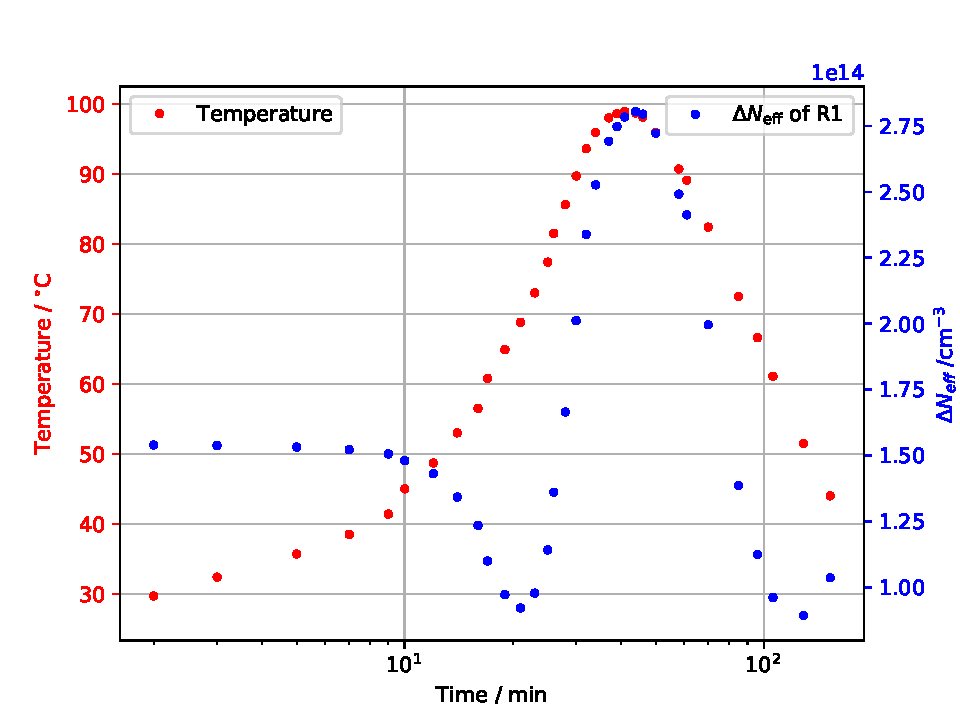
\includegraphics[width=0.49\textwidth]{images/ohnekorrektur.PDF}}
      \subfigure[]{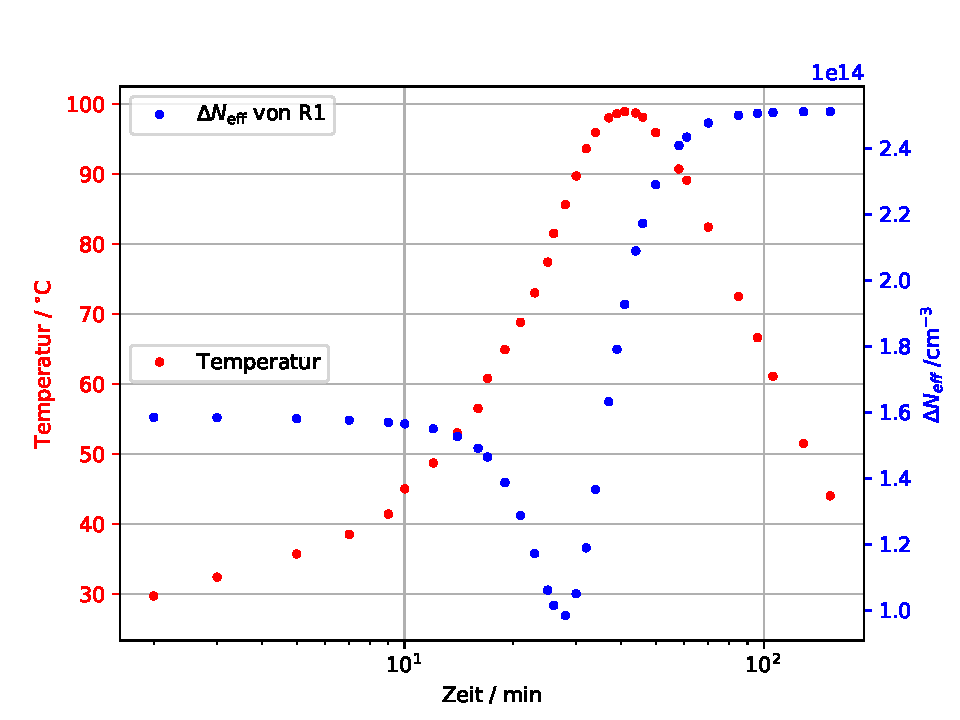
\includegraphics[width=0.49\textwidth]{images/annealingtdata.PDF}}
  \caption{$\Delta N_{eff}$ des Sensors R1 ohne Korrektur (a) und mit Korrektur (b) nach einer Bestrahlung mit Fluenz $\Phi_{\mathrm{eq}} = \SI{5e15}{\per\centi\meter\squared}.$}
  \end{figure}
\end{frame}

\begin{frame}{Schadensrate mit Korrektur}
  \begin{itemize}
    \item Korrektur funktioniert
    \medskip
    \item Analoger Ansatz für die Schadensrate
    \medskip
    \item Korrektur von $\frac{t}{\tau_{\mathrm{I}}(T)}$ und  $\Theta(T) \cdot t$
    \medskip
    \item Schadensrate kann beim annealing nur sinken
  \end{itemize}
\end{frame}

\begin{frame}{Schadensrate mit Korrektur}
  \begin{figure}
        \subfigure[]{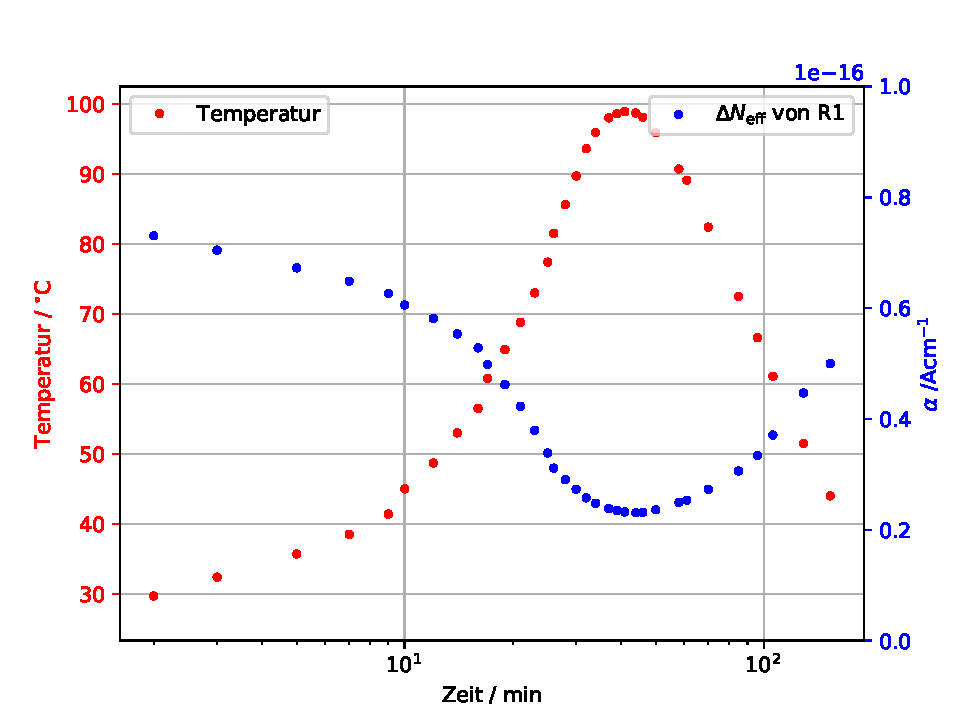
\includegraphics[width=0.49\textwidth]{images/damage_ohne_korrektur.PDF}}
        \subfigure[]{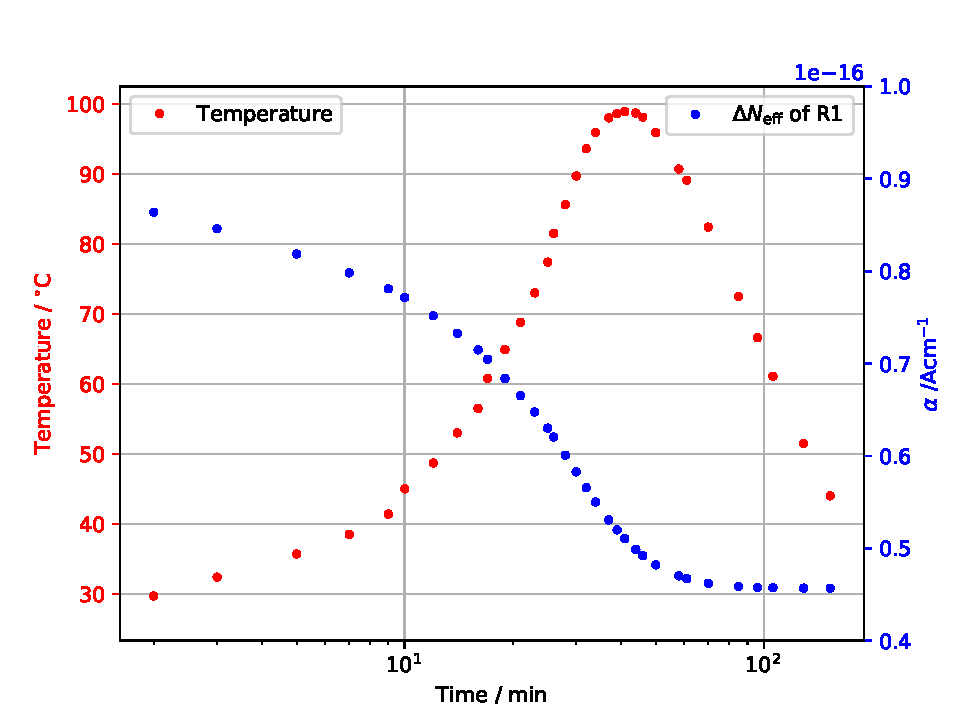
\includegraphics[width=0.49\textwidth]{images/damagekorrektur.PDF}}
  \caption{Schadensrate des Sensors R1 ohne Korrektur (a) und mit Korrektur (b).}
  \end{figure}
\end{frame}


\begin{frame}{Interpolation der Daten}
  Auftrendes Problem: Große Zeitabstände zwischen Messwerten führen zu Ungenauigkeiten
  \medskip

  $\rightarrow$ Lineare Interpolation der Temperaturkurve
  \medskip
  \begin{itemize}
    \item Anzahl $n$ der Intervalle der linearen Interpolation zwischen den Zeiten $t_{\mathrm{A}}$ und $t_{\mathrm{B}}$ :
    \begin{align*}
      n = \left\lceil y \cdot \frac{T_{\mathrm{i}}-T_{\mathrm{i+1}}}{T_{\mathrm{max}}-T_{\mathrm{i}}+ z_1}+z_2 \right\rceil
    \end{align*}

    \item Interpolierte Zeit und Temperatur zwischen $t_{\mathrm{A}}$ und $t_{\mathrm{B}}$:
    \begin{align*}
      t_i &= t_{\mathrm{A}} +  \frac{t_{\mathrm{B}}-t_{\mathrm{A}}}{n} \cdot i \\
      T_i &= T_{\mathrm{A}} +  \frac{T_{\mathrm{B}}-T_{\mathrm{A}}}{n} \cdot i \\
      i &= 1, 2, ..., n
    \end{align*}
  \end{itemize}
\end{frame}

\begin{frame}{Interpolierte Temperatur}
  \begin{figure}
      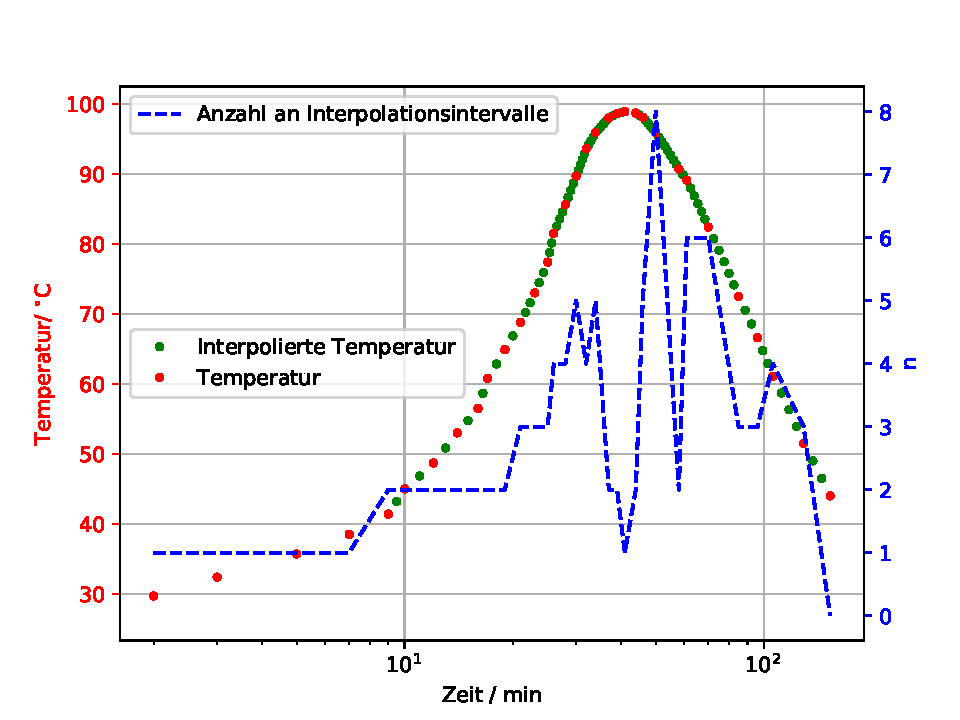
\includegraphics[width=0.55\textwidth]{images/interpolation_steps.PDF}
  \caption{Interpolierte Temperatur mit Parametern $y=15$, $z_1=5^\circ$C und $z_2 = 0.2$.}
  \end{figure}
\end{frame}

\begin{frame}{Interpolation der Dotierungskonzentration}
  \begin{figure}
      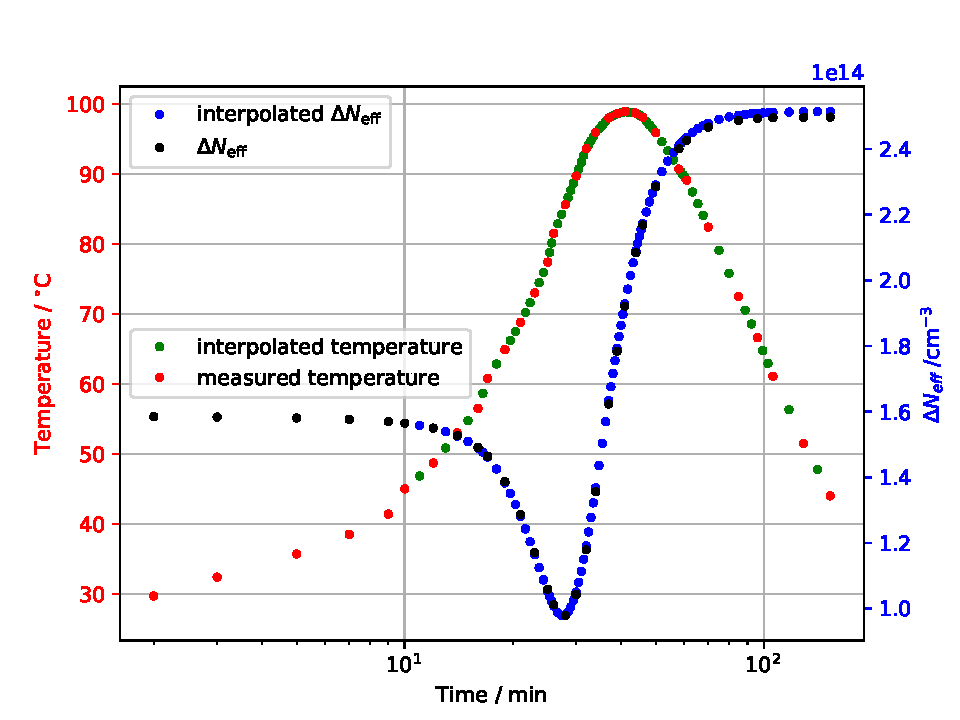
\includegraphics[width=0.55\textwidth]{images/interpolationtdata.PDF}
  \caption{Interpolierte Temperatur und $\Delta N_{\mathrm{eff}}$.}
  \end{figure}
\end{frame}


\begin{frame}{Interpolation der Schadensrate}
  \begin{figure}
      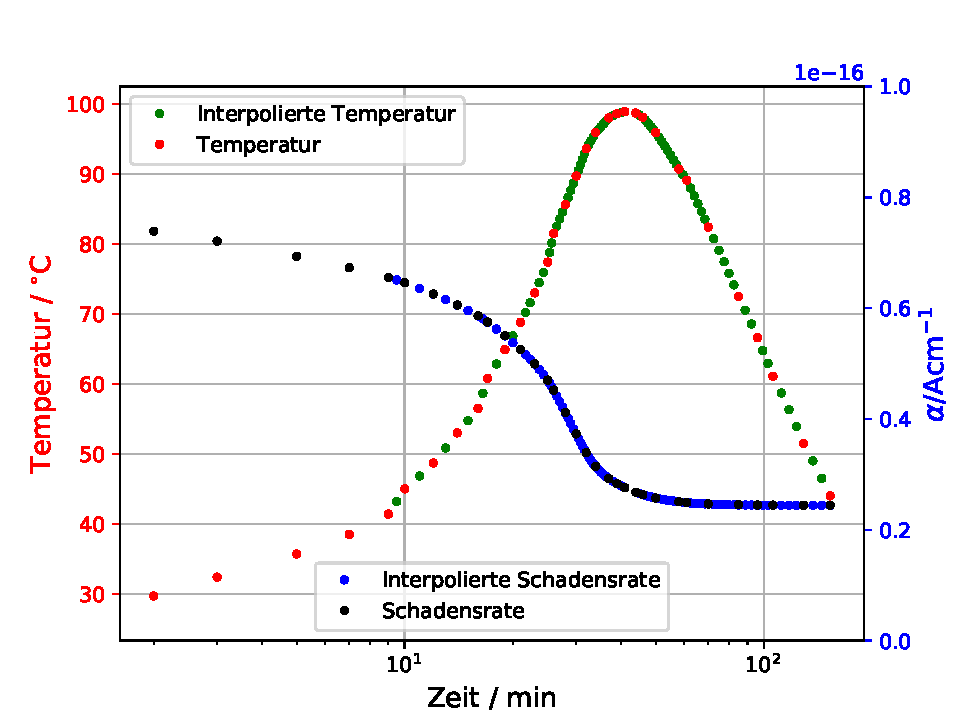
\includegraphics[width=0.55\textwidth]{images/damage_interpolation.PDF}
  \caption{Interpolierte Temperatur und Schadensrate.}
  \end{figure}
\end{frame}

\begin{frame}{Annealinghistorie}
  \begin{itemize}
    \item Darstellung einer gesamten Annealinghistorie eines Sensors durch Verknüpfung aller Daten
  \end{itemize}

  \begin{figure}
      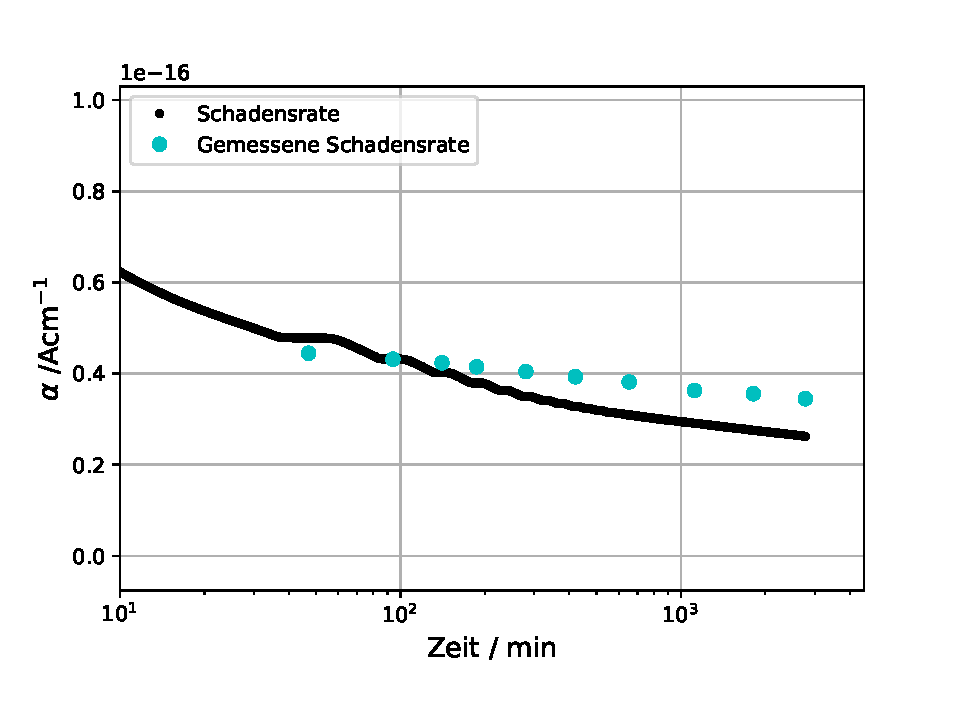
\includegraphics[width=0.53\textwidth]{images/damage_P_3.PDF}
  \caption{Theoretische und gemessene Schadensrate.}
  \end{figure}
\end{frame}

\begin{frame}{Abweichungen}
  \begin{itemize}
    \item Parameter der Funktion entsprechen nicht den Parametern des Sensors
    \medskip
    \item Sensor wurde schon vorher annealed
    \medskip
    \item Messwerte unterliegen systematischen Unsicherheiten
    \medskip
    \begin{itemize}
      \item Volumen des Sensormaterials
      \medskip
      \item Leckstrom
    \end{itemize}
  \end{itemize}
\end{frame}

\begin{frame}{Interface}
  \begin{itemize}
    \item Erstellung eines Interfaces für schnelle Berechnungen von $N_{\mathrm{eff}}$ und $\alpha$
    \item Modellierung für beliebige Annealingzeiten, Fluenzen und konstante Temperaturen
  \end{itemize}
  \begin{figure}
      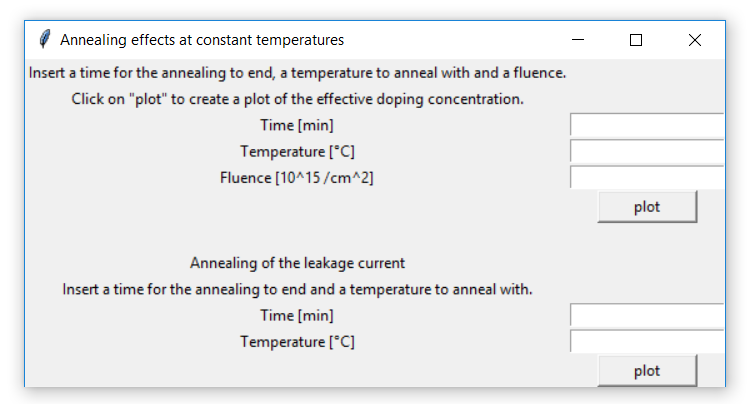
\includegraphics[width=0.53\textwidth]{images/interface.PNG}
  \caption{Interface zur Berechnung von $N_{\mathrm{eff}}$ und $\alpha$.}
  \end{figure}
\end{frame}

\begin{frame}{Interface Beispiel: Dotierungskonzentration}
  \begin{figure}
    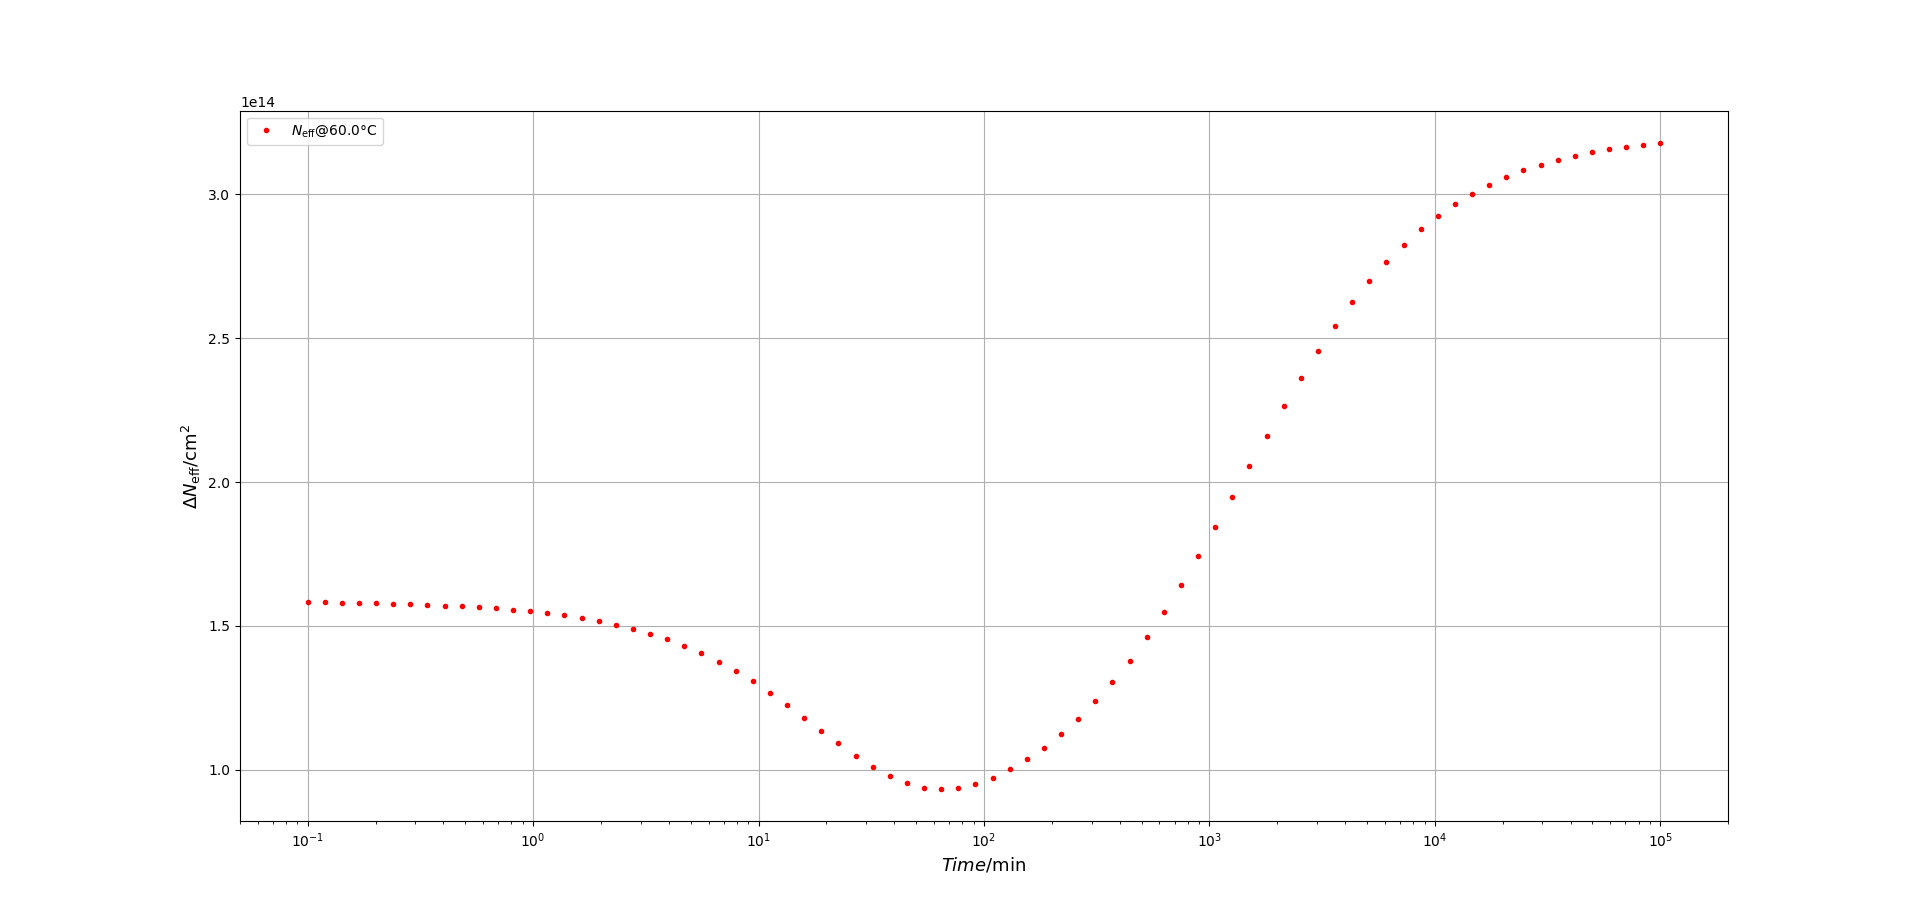
\includegraphics[width=0.55\textwidth]{images/interface_n_eff.PDF}
    \caption{Beispiel Plot von $N_{\mathrm{eff}}$ mit $t = \SI{10e5}{\minute}$, $\Phi_{\mathrm{eq}}= \SI{5e15}{\per\centi\meter\squared}$}
  \end{figure}
\end{frame}

\begin{frame}{Interface Beispiel: Schadensrate}
  \begin{figure}
    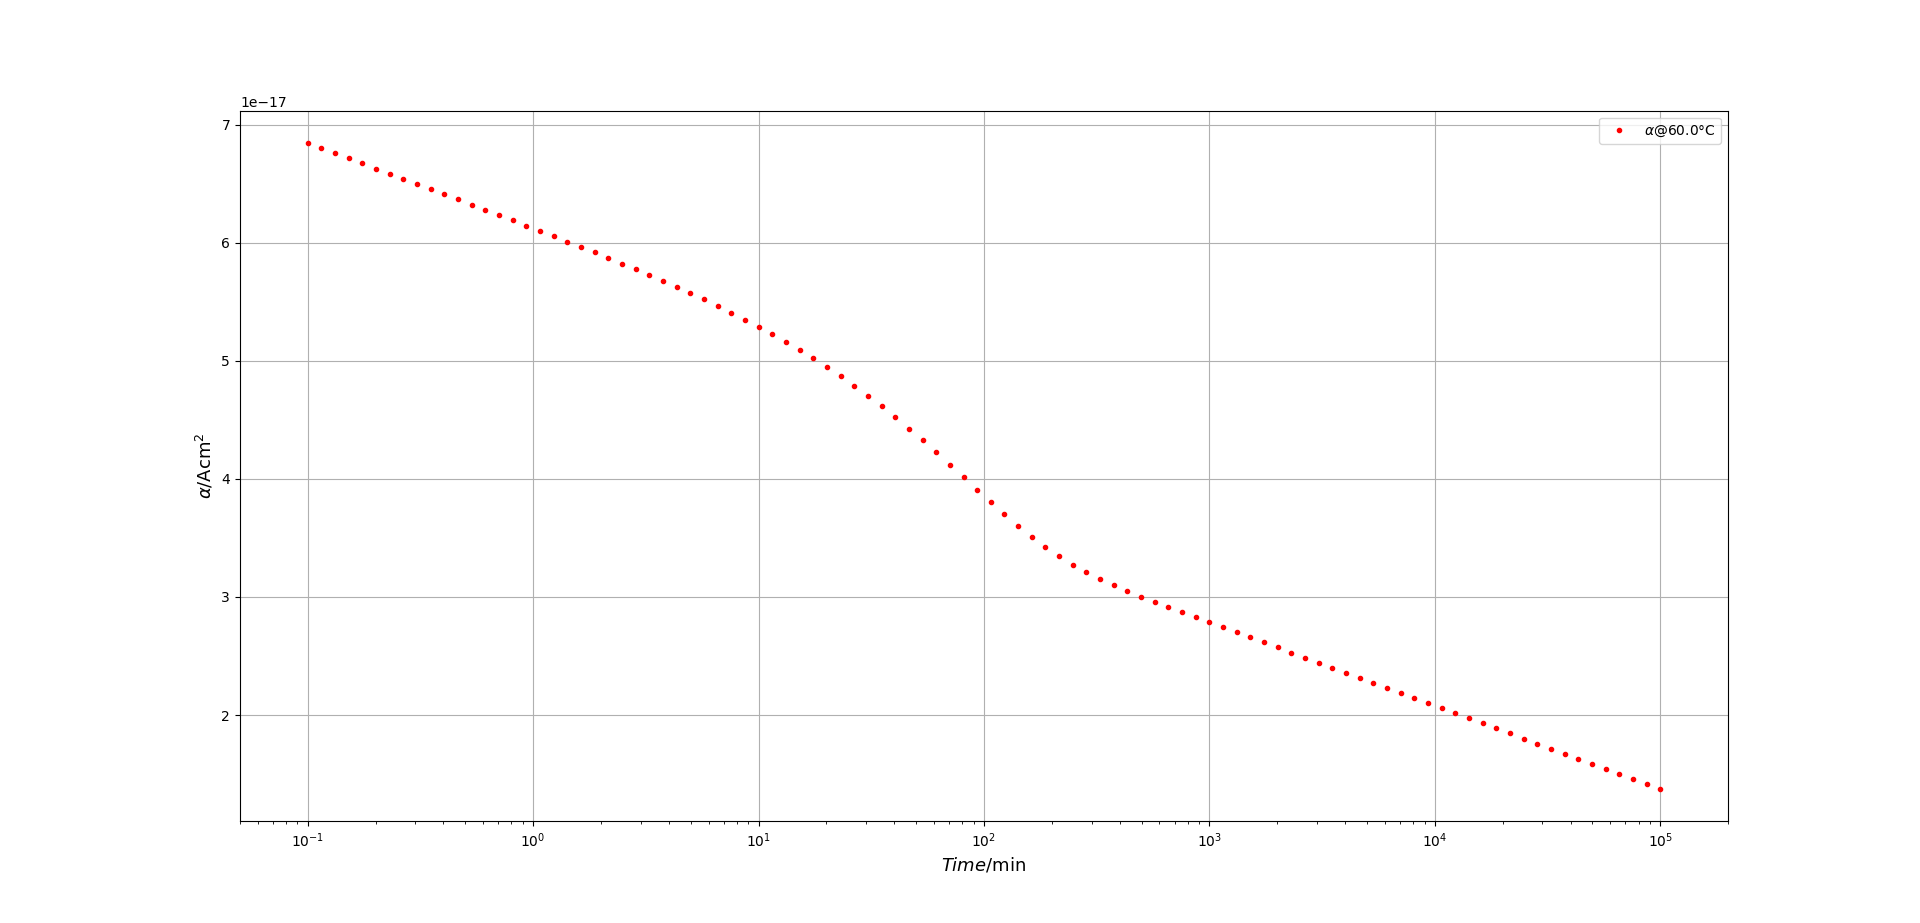
\includegraphics[width=0.55\textwidth]{images/interface_damage.PDF}
    \caption{Beispiel Plot von $\alpha$ mit $t = \SI{10e5}{\minute}$}
  \end{figure}
\end{frame}

\begin{frame}{Fazit}
  \begin{itemize}
    \item Funktionsfähiges Programm zur Berechnung von $N_{\mathrm{eff}}$ und $\alpha$
    \medskip
    \item Inklusive eines Programms zur Verbindung von Datendateien und Anpassung der Zeiten
    \medskip
    \item Parameter, anzeigbares Verhalten bei konstanter Temperatur und Anzahl an Interpolationsintervallen in den
    Einstellungen wählbar.
    \medskip
    \item Anleitung zur Bedienung des Programms vorhanden
    \medskip
    \item Interface zum Modellieren für konstante Temperaturen mit einstellbaren Parametern
  \end{itemize}
\end{frame}

\end{document}
